\chapter{Σύνολα Δεδομένων}
\label{ch:datasets}

\section{Εισαγωγή}
\label{sec:datasets-introduction}

Η πειραματική διερεύνηση των διαφορετικών στρατηγικών απόσταξης γνώσης,
οι οποίες περιγράφονται αναλυτικά στο Κεφάλαιο~\ref{ch:implementation},
πραγματοποιείται με τη χρήση των \tl{HMDB51} και \tl{UCF101}, δύο
καθιερωμένων συνόλων αναφοράς (\tl{benchmarks}) για την αναγνώριση
ανθρώπινων ενεργειών σε βίντεο. Το \tl{HMDB51} αποτελεί το βασικό
σύνολο δεδομένων της εργασίας, ενώ το \tl{UCF101} χρησιμοποιείται
συμπληρωματικά σε επιλεγμένα πειράματα, περιλαμβάνοντας μεγαλύτερο
αριθμό βίντεο και κλάσεων.

Και τα δύο σύνολα αποτελούνται από σύντομα αποσπάσματα βίντεο σε μορφή
αρχείων \tl{AVI}, ενώ οι κλάσεις τους οργανώνονται σε πέντε ευρύτερες
κατηγορίες ενεργειών. Τα βίντεο έχουν καταγραφεί σε μη ελεγχόμενες
συνθήκες και παρουσιάζουν σημαντικές διαφοροποιήσεις ως προς την
ποιότητα, την κίνηση της κάμερας, την οπτική γωνία, το φόντο και τον
φωτισμό. Επιπλέον, παρέχουν τρεις επίσημους διαχωρισμούς (\tl{splits})
σε σύνολο εκπαίδευσης (\tl{training set}) και σύνολο ελέγχου
(\tl{test set}), από τους οποίους στην παρούσα εργασία χρησιμοποιείται ο
πρώτος (\tl{split 1}).

\section{\tl{HMDB51}}
\label{sec:hmdb51-dataset}

Το \tl{HMDB51} περιλαμβάνει συνολικά 6.766 αποσπάσματα βίντεο από
51 κλάσεις ανθρώπινων ενεργειών \cite{kuehne2011hmdb}, τα οποία
προέρχονται κυρίως από κινηματογραφικές ταινίες και διαδικτυακές πηγές.

Στον πρώτο επίσημο διαχωρισμό επιλέγονται, για καθεμία από τις 51
κλάσεις, 70 βίντεο για εκπαίδευση και 30 για έλεγχο. Προκύπτουν έτσι
3.570 βίντεο εκπαίδευσης και 1.530 βίντεο ελέγχου, ενώ τα υπόλοιπα
1.666 βίντεο της αρχικής συλλογής δεν συμμετέχουν στον συγκεκριμένο
διαχωρισμό.

\section{\tl{UCF101}}
\label{sec:ucf101-dataset}

Μεγαλύτερο σε κλίμακα είναι το \tl{UCF101}, το οποίο περιλαμβάνει
13.320 αποσπάσματα βίντεο από 101 κλάσεις ανθρώπινων ενεργειών
\cite{soomro2012ucf101}. Σε αντίθεση με το \tl{HMDB51}, το υλικό του
έχει συλλεχθεί αποκλειστικά από το \tl{YouTube}.

Ο πρώτος επίσημος διαχωρισμός περιλαμβάνει 9.537 βίντεο εκπαίδευσης και
3.783 βίντεο ελέγχου. Επειδή ο αριθμός των βίντεο διαφέρει μεταξύ των
κλάσεων, τα σύνολα εκπαίδευσης και ελέγχου δεν είναι ισορροπημένα ως προς
τις κλάσεις.
\section{Σύγκριση των συνόλων δεδομένων}
\label{sec:dataset-comparison}

Οι δύο συλλογές παρουσιάζουν περιορισμένη θεματική επικάλυψη. Ειδικότερα,
στη βιβλιογραφία έχουν αντιστοιχιστεί 12 κοινές κατηγορίες ενεργειών
μεταξύ των \tl{HMDB51} και \tl{UCF101} \cite{chen2019temporal}, οι οποίες
αφορούν κυρίως κινήσεις του σώματος και αθλητικές δραστηριότητες. Πέρα από
αυτή την περιορισμένη επικάλυψη, οι ευρύτερες θεματικές κατηγορίες των δύο
συλλογών δεν βρίσκονται σε πλήρη αντιστοιχία, καθώς το \tl{HMDB51}
διακρίνει ειδικότερα τις ενέργειες του προσώπου, ενώ το \tl{UCF101}
περιλαμβάνει ξεχωριστές ομάδες για τις αθλητικές δραστηριότητες και το
παίξιμο μουσικών οργάνων. Οι κατηγορίες αυτές, μαζί με το πλήθος των
κλάσεων που περιλαμβάνει η καθεμία, συνοψίζονται στον
Πίνακα~\ref{tab:dataset-action-groups}.

\begin{table}[H]
    \centering
    \caption{Κατανομή των κλάσεων των \tl{HMDB51} και \tl{UCF101} στις
        ευρύτερες κατηγορίες ενεργειών.}
    \label{tab:dataset-action-groups}
    \small
    \begin{tabular}{llc}
        \hline
        \textbf{Σύνολο δεδομένων} & \textbf{Ευρύτερη κατηγορία} & \textbf{Κλάσεις} \\
        \hline
        \tl{HMDB51} & Γενικές ενέργειες του προσώπου & 4 \\
                    & Ενέργειες του προσώπου με χειρισμό αντικειμένων & 3 \\
                    & Γενικές κινήσεις του σώματος & 19 \\
                    & Κινήσεις του σώματος με αλληλεπίδραση με αντικείμενα & 18 \\
                    & Αλληλεπιδράσεις μεταξύ ανθρώπων & 7 \\
        \hline
        \tl{UCF101} & Αλληλεπίδραση ανθρώπου με αντικείμενα & 20 \\
                    & Κινήσεις του σώματος & 16 \\
                    & Αλληλεπίδραση μεταξύ ανθρώπων & 5 \\
                    & Εκτέλεση μουσικών οργάνων & 10 \\
                    & Αθλητικές δραστηριότητες & 50 \\
        \hline
    \end{tabular}
\end{table}

Καθώς μία κοινή κατηγορία μπορεί να αντιστοιχεί σε περισσότερες από μία
κλάσεις του \tl{UCF101}, η πλήρης αντιστοίχιση παρουσιάζεται στον
Πίνακα~\ref{tab:hmdb-ucf-common-classes}.

\begin{table}[H]
    \centering
    \caption{Αντιστοίχιση των κλάσεων των \tl{HMDB51} και \tl{UCF101} στις
κοινές κατηγορίες ενεργειών \cite{chen2019temporal}.}
    \label{tab:hmdb-ucf-common-classes}
    \small
    \begin{tabular}{lll}
        \hline
        \textbf{Κοινή κατηγορία} & \textbf{\tl{HMDB51}} & \textbf{\tl{UCF101}} \\
        \hline
        \tl{Climb}      & \tl{climb}       & \tl{RockClimbingIndoor}, \tl{RopeClimbing} \\
        \tl{Fencing}    & \tl{fencing}     & \tl{Fencing} \\
        \tl{Golf}       & \tl{golf}        & \tl{GolfSwing} \\
        \tl{Kick ball}  & \tl{kick\_ball}  & \tl{SoccerPenalty} \\
        \tl{Pull-up}    & \tl{pullup}      & \tl{PullUps} \\
        \tl{Punch}      & \tl{punch}       & \tl{Punch}, \tl{BoxingPunchingBag}, \tl{BoxingSpeedBag} \\
        \tl{Push-up}    & \tl{pushup}      & \tl{PushUps} \\
        \tl{Ride bike}  & \tl{ride\_bike}  & \tl{Biking} \\
        \tl{Ride horse} & \tl{ride\_horse} & \tl{HorseRiding} \\
        \tl{Shoot ball} & \tl{shoot\_ball} & \tl{Basketball} \\
        \tl{Shoot bow}  & \tl{shoot\_bow}  & \tl{Archery} \\
        \tl{Walk}       & \tl{walk}        & \tl{WalkingWithDog} \\
        \hline
    \end{tabular}
\end{table}


Τα στατιστικά στοιχεία των βίντεο του πρώτου επίσημου διαχωρισμού
συνοψίζονται στον Πίνακα~\ref{tab:dataset-comparison}.

\begin{table}[H]
    \centering
    \caption{Χαρακτηριστικά των \tl{HMDB51} και \tl{UCF101} στον πρώτο
επίσημο διαχωρισμό.}
    \label{tab:dataset-comparison}
    \begin{tabular}{lcc}
        \hline
        \textbf{Χαρακτηριστικό} &
        \textbf{\tl{HMDB51}} &
        \textbf{\tl{UCF101}} \\
        \hline
        Πλήθος κλάσεων & 51 & 101 \\
        Βίντεο που συμμετέχουν & 5.100 & 13.320 \\
        Βίντεο εκπαίδευσης & 3.570 & 9.537 \\
        Βίντεο ελέγχου & 1.530 & 3.783 \\
        Βίντεο εκπαίδευσης ανά κλάση & 70 & 72--121 \\
        Βίντεο ελέγχου ανά κλάση & 30 & 28--49 \\
        Ισορροπημένος διαχωρισμός ανά κλάση & Ναι & Όχι \\
        Μέση διάρκεια (\tl{s}) & 3,23 & 7,21 \\
        Διάμεση διάρκεια (\tl{s}) & 2,67 & 6,48 \\
        Ελάχιστη διάρκεια (\tl{s}) & 0,63 & 1,07 \\
        Μέγιστη διάρκεια (\tl{s}) & 35,43 & 71,04 \\
        Ρυθμός καρέ (\tl{fps}) & 30 & 25 \\
        Ανάλυση (\tl{pixels}) &
\(176\text{--}592 \times 240\) &
\(320\times240\) \\
        \hline
    \end{tabular}
\end{table}

Τέλος, ενδεικτικά βίντεο από διαφορετικές κλάσεις των δύο συνόλων παρουσιάζονται στα Σχήματα~\ref{fig:hmdb51-sample-frames} και~\ref{fig:ucf101-sample-frames}.

\begin{figure}[H]
    \centering
    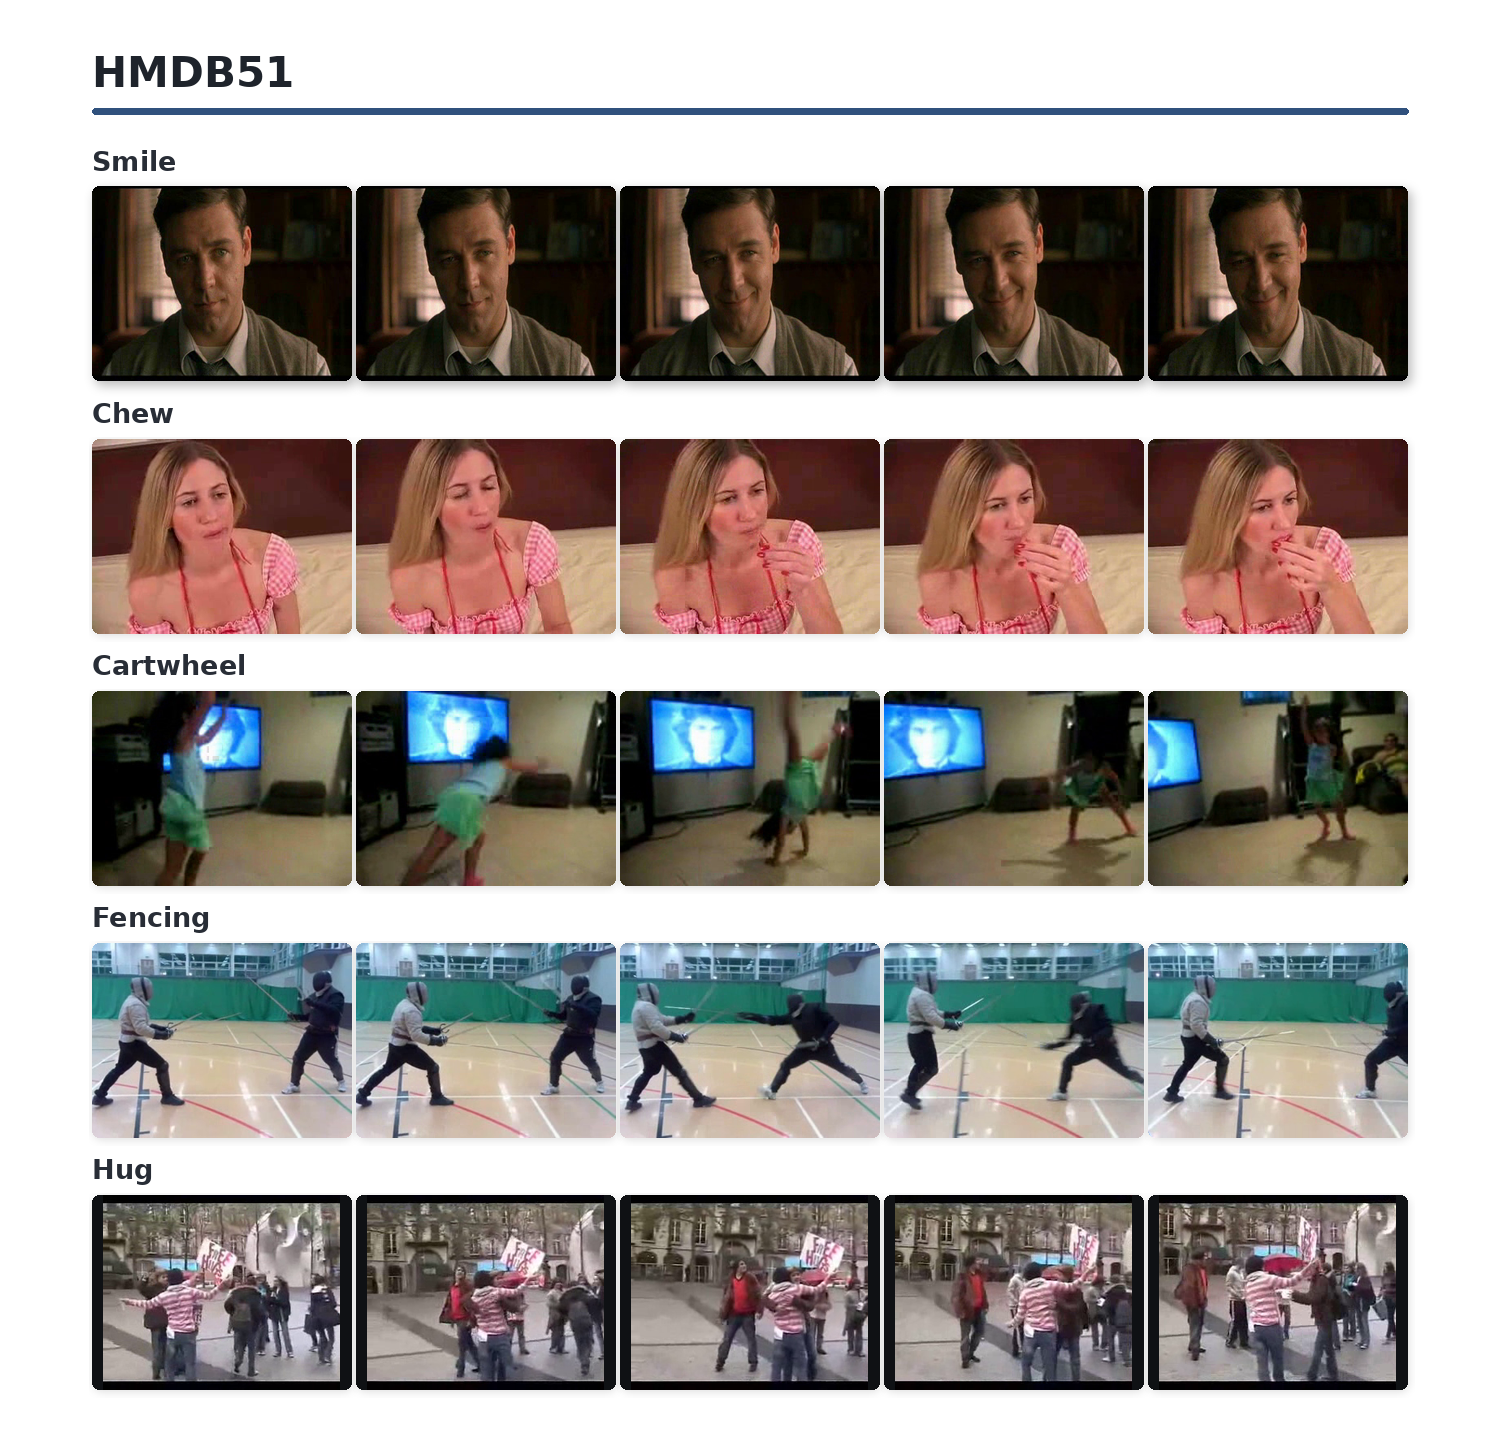
\includegraphics[width=\textwidth]{hmdb51_sample_storyboards.png}
    \caption{Παραδείγματα από πέντε κλάσεις του \tl{HMDB51}. Σε κάθε σειρά
παρουσιάζονται πέντε ομοιόμορφα κατανεμημένα καρέ ενός βίντεο.}
    \label{fig:hmdb51-sample-frames}
\end{figure}

\begin{figure}[H]
    \centering
    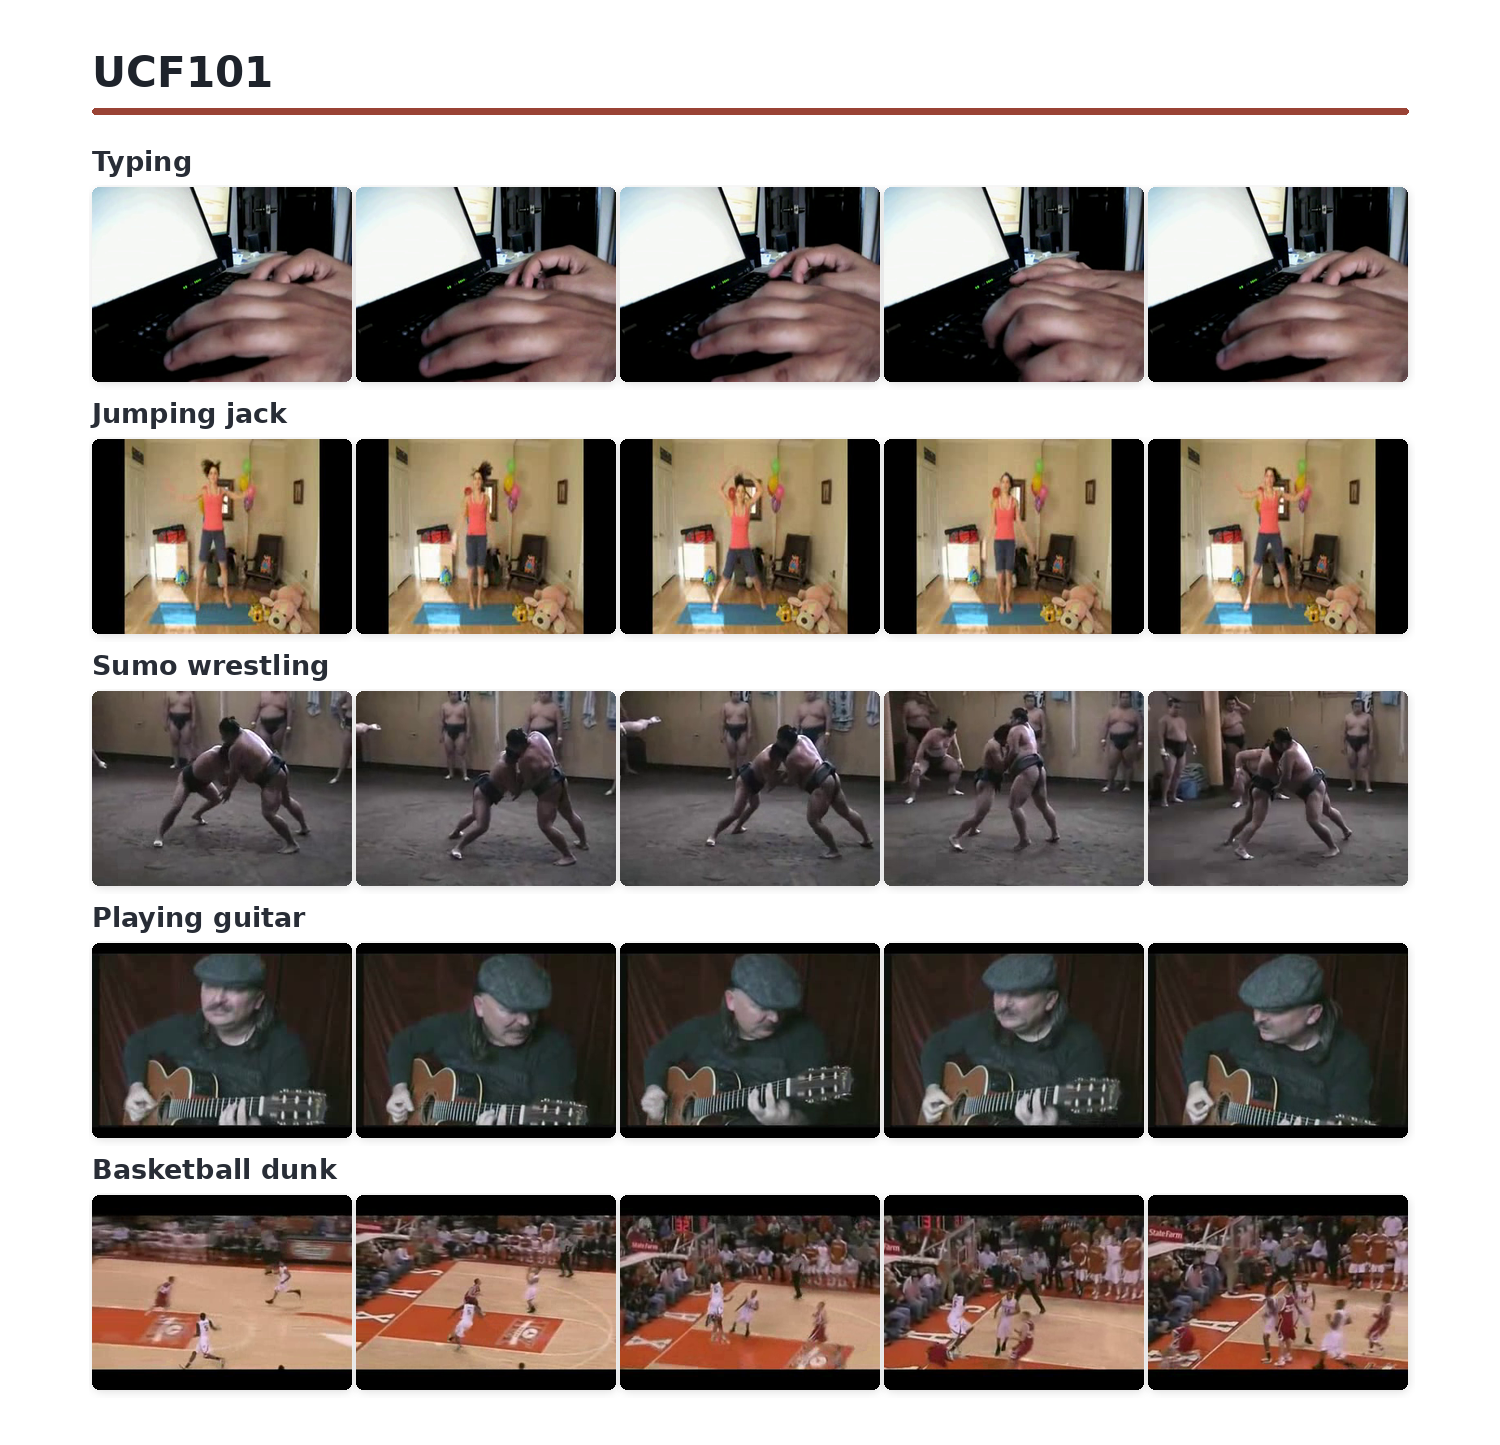
\includegraphics[width=\textwidth]{ucf101_sample_storyboards.png}
    \caption{Παραδείγματα από πέντε κλάσεις του \tl{UCF101}. Σε κάθε σειρά
παρουσιάζονται πέντε ομοιόμορφα κατανεμημένα καρέ ενός βίντεο.}
    \label{fig:ucf101-sample-frames}
\end{figure}

\section{Ρόλος των συνόλων δεδομένων στην πειραματική διαδικασία}
\label{sec:dataset-usage}

Στη σχετική βιβλιογραφία, η απόσταξη γνώσης σε μοντέλα βίντεο έχει
εφαρμοστεί σε σύνολα δεδομένων μεγάλης κλίμακας. Χαρακτηριστικό
παράδειγμα αποτελεί η μέθοδος \tl{MVD} \cite{wang2023mvd}, στην οποία η
απόσταξη πραγματοποιείται στο \tl{Kinetics-400}
\cite{kay2017kinetics}, ένα σύνολο που περιλαμβάνει εκατοντάδες χιλιάδες
βίντεο. Ωστόσο, στην παρούσα εργασία η χρήση ενός συνόλου τέτοιας
κλίμακας κρίθηκε πρακτικά ανέφικτη με βάση τους διαθέσιμους
υπολογιστικούς πόρους και το χρονικό πλαίσιο εκπόνησής της. Επιπλέον, η
πειραματική μελέτη περιλαμβάνει τρεις στρατηγικές απόσταξης, τρεις
αρχιτεκτονικές-\tl{student} και πολλαπλές παραλλαγές των
υπερπαραμέτρων τους, γεγονός που απαιτεί την εκτέλεση μεγάλου αριθμού
πειραμάτων και αυξάνει περαιτέρω το συνολικό υπολογιστικό κόστος.

Για τους λόγους αυτούς, επιλέχθηκαν τα μικρότερα σύνολα δεδομένων
\tl{HMDB51} και \tl{UCF101}. Κατά τα στάδια της απόσταξης, οι διαθέσιμες
ετικέτες των κλάσεων δεν συμμετέχουν στις συναρτήσεις απώλειας, καθώς οι
στόχοι εκπαίδευσης προκύπτουν από τις εξόδους του
μοντέλου-\tl{teacher}. Οι ετικέτες αξιοποιούνται στα επιβλεπόμενα στάδια
εκπαίδευσης και στον υπολογισμό των μετρικών αξιολόγησης.

Το \tl{HMDB51} αποτελεί το βασικό σύνολο δεδομένων της εργασίας. Αρχικά,
χρησιμοποιείται για την εκπαίδευση του \tl{attentive classifier} του
μοντέλου-\tl{teacher}. Στη συνέχεια, αξιοποιείται ως σύνολο απόσταξης
σε όλες τις στρατηγικές, για τη μεταφορά γνώσης από το
μοντέλο-\tl{teacher} στα μικρότερα μοντέλα-\tl{student}, καθώς και για
την επιβλεπόμενη εκπαίδευση των \tl{attentive classifiers} στο δεύτερο
στάδιο της στρατηγικής απόσταξης δύο σταδίων.
Επιπλέον, χρησιμοποιείται για την επιβλεπόμενη εκπαίδευση των
μοντέλων-\tl{student} από την αρχή, ώστε να προκύψουν τα αποτελέσματα
αναφοράς (\tl{supervised baselines}) με τα οποία συγκρίνονται τα
αντίστοιχα αποσταγμένα μοντέλα. Η τελική αξιολόγηση όλων των μοντέλων
πραγματοποιείται στο σύνολο ελέγχου του \tl{HMDB51}.

Το \tl{UCF101} χρησιμοποιείται συμπληρωματικά, μόνο στο πρώτο στάδιο της
στρατηγικής απόσταξης δύο σταδίων, δηλαδή στην απόσταξη του
\tl{backbone}, με σκοπό να διερευνηθεί κατά πόσο η χρήση μεγαλύτερου
πλήθους βίντεο μπορεί να βελτιώσει τη μεταφορά των αναπαραστάσεων από
το μοντέλο-\tl{teacher} στο μοντέλο-\tl{student}. Με τον τρόπο αυτό εξετάζεται τόσο η απόσταξη σε δεδομένα της ίδιας
κατανομής με το σύνολο αξιολόγησης όσο και η μεταφορά αναπαραστάσεων από
ένα διαφορετικό αλλά συναφές σύνολο βίντεο. Στο ίδιο στάδιο
εξετάζεται επίσης ένα μικτό σύνολο δεδομένων, το οποίο συνδυάζει βίντεο
από τα \tl{HMDB51} και \tl{UCF101}. Στην πρώτη παραλλαγή
χρησιμοποιούνται όλα τα διαθέσιμα βίντεο εκπαίδευσης των δύο συλλογών,
ενώ στη δεύτερη περιορίζεται μέσω δειγματοληψίας ο αριθμός των βίντεο
του \tl{UCF101}, ώστε οι δύο συλλογές να συνεισφέρουν περίπου τον ίδιο
αριθμό δειγμάτων. Σε όλες τις περιπτώσεις, το δεύτερο στάδιο, δηλαδή η
εκπαίδευση του \tl{attentive classifier}, πραγματοποιείται στο
\tl{HMDB51}.

Για τις ανάγκες των πειραμάτων, το επίσημο σύνολο εκπαίδευσης κάθε
συλλογής διαχωρίζεται περαιτέρω σε ένα εσωτερικό σύνολο εκπαίδευσης και
ένα σύνολο επικύρωσης (\tl{validation set}). Η διαδικασία δημιουργίας των
υποσυνόλων αυτών, καθώς και η δειγματοληψία των καρέ και τα
στάδια προεπεξεργασίας, περιγράφονται στο επόμενο κεφάλαιο.
